
\documentclass{article}
\usepackage[utf8]{inputenc}
\usepackage{fancyhdr}
\pagestyle{fancy}
\lhead{CRI Report Generator}
\rhead{UIC Center for Research Informatics}
\rfoot{page \thepage}
\lfoot{ \date{ }}
\renewcommand{\headrulewidth}{0.4pt}
\renewcommand{\footrulewidth}{0.4pt}
\usepackage{tikz}
\usetikzlibrary{shapes.misc}

\tikzset{cross/.style={cross out, draw=black, minimum size=2*(#1-\pgflinewidth), inner sep=0pt, outer sep=0pt},
%default radius will be 1pt. 
cross/.default={1pt}}


\usepackage{listings}
\usepackage{color}

\definecolor{dkgreen}{rgb}{0,0.6,0}
\definecolor{gray}{rgb}{0.5,0.5,0.5}
\definecolor{mauve}{rgb}{0.58,0,0.82}

\lstset{frame=tb,
  language=Java,
  aboveskip=3mm,
  belowskip=3mm,
  showstringspaces=false,
  columns=flexible,
  basicstyle={\small\ttfamily},
  numbers=none,
  numberstyle=\tiny\color{gray},
  keywordstyle=\color{blue},
  commentstyle=\color{dkgreen},
  stringstyle=\color{mauve},
  breaklines=true,
  breakatwhitespace=true,
  tabsize=3
}
 
\title{CRI Report Generator}
\author{Gobind Singh}
\date{ }
 
\begin{document}
 
\maketitle
 
\tableofcontents
 
\section{Requirements}
 
The Center for Research Informatics (CRI) requires a report generation script to automatically summarize the process and results of its analysis.  The solution should fullfill the following requirements:
\begin{enumerate}
    \item Pull in configuration file information into the output report file.
    \item Validate predefined set memberships, alert if not valid. 
    \item Embed linked figures (jpg,png,pdf), data(bam,fastq), and tables(csv) into the report.
    \item Formating table of contents, citations, and sections.
    \item Styling such as logo, title, and date. 
\end{enumerate}

 
\section{Design Overview}
The CRI Report Generator solution will rely on XSLT, to transform xml report and configuration files to the required html output format.  XSLT is domain specific to XML and supports XPath to select DOM elements.  XSLT is the ideal solution for static html generation from xml and configuration files.  An XML schema can be created to allow authors to write the report content in a simplified manner.  Further, the xml schema can be validated by xslt, which can assert errors.  Finally, CSS can be used for styling of html elements.  


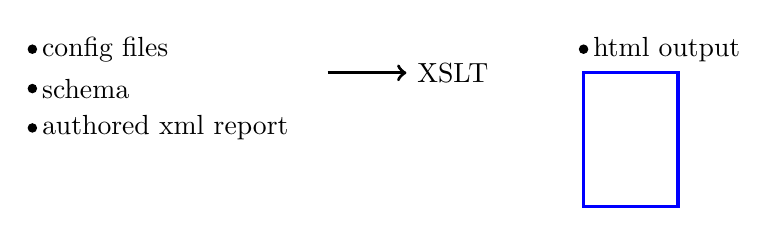
\begin{tikzpicture}
\filldraw[black] (0,2.5) circle (1.5pt) node[anchor=west] {config files};
\filldraw[black] (0,2) circle (1.5pt) node[anchor=west] {schema};
\filldraw[black] (0,1.5) circle (1.5pt) node[anchor=west] {authored xml report};

\draw[very thick,->] (3.75,2.2) -- (4.75,2.2) node[anchor=west] {XSLT};

\draw[blue, very thick] (7,0.5)rectangle (8.2,2.2);
\filldraw[black] (7,2.5) circle (1.5pt) node[anchor=west] {html output};
\end{tikzpicture}


\addcontentsline{toc}{section}{\protect\numberline{}Scope}%
\section*{Scope}
The main limitation of this approach is in attempts to use in web applications.  For the purpose of serving html files a standard web solution should be found.  For the purpose of transforming xml to html, xslt is the standard solution.  

\section{Implementation}
There exist free xslt editors such as Treebeard (http://treebeard.sourceforge.net/) and non-free Oxygen (http://www.oxygenxml.com/).  The Saxon xslt processor runs in both.   

XSLT can be used to generate table of contents, numbered citations, and link to configuration files.

Configuration files will be written in xml; as will the authored report files.

Relax NG, a schema language for xml.  It can be used to validate authored xml files.  For more complicated validation, such as asserting set membership, Schematron, an xml schema language which finds tree patterns in parsed documents, can be used. 

CSS, cascading style sheets, is the standard for styling of sections. 

\begin{lstlisting}
// Hello.java
import javax.swing.JApplet;
import java.awt.Graphics;

public class Hello extends JApplet {
    public void paintComponent(Graphics g) {
        g.drawString("Hello, world!", 65, 95);
    }    
}
\end{lstlisting}



\end{document}


